\subsection{Berekening ideale overbrenging}
\label{bijlage:overbrenging}
Wanneer de rover in beweging is, werken er in totaal drie krachten op in. Deze krachten zijn de voortdrijvende kracht door de motor, de wrijvingskracht door de rolweerstand en de wrijvingskracht door de luchtweerstand. De bewegingsvergelijking is dus:
\begin{equation} \label{eq:diff_vgl}
F_{motor}-F_{rol}-F_{lucht} = m*a
\end{equation}
De wrijvingskracht door de rolweerstand wordt bepaald met behulp van de volgende vergelijking.
\begin{equation} \label{eq:rolweerstand}
F_{rol}=\mu*m*g
\end{equation}
De wrijvingskracht door de luchtweerstand wordt bepaald met behulp van deze vergelijking.
%Hierin stelt A de oppervlakte voor die weerstand ondervindt door de lucht. De dichtheid van de lucht wordt voorgesteld door lucht en de snelheid van de rover door v.
\begin{equation} \label{eq:luchtweerstand}
F_{lucht}=\frac{1}{2} * \rho_{lucht} * Cd * A * v^2
\end{equation}
De aandrijvende kracht van de motor wordt verkregen met behulp van de volgende formule.
\begin{equation} \label{eq:motor}
F_{motor}=\frac{\eta}{R_{wiel}} * \frac{T_{max}-\left(T_{max}*\frac{dx}{dt}\right)}{\omega_{max}*R_{wiel}}
\end{equation}
Door vergelijkingen ~\ref{eq:rolweerstand},~\ref{eq:luchtweerstand} en ~\ref{eq:motor} in te vullen in vergelijking ~\ref{eq:diff_vgl} kan de vergelijking volledig opgelost worden. Als beginvoorwaarden wordt de snelheid en de plaats van de wagen op tijdstip 0 gelijk gesteld aan 0. De oplossing van de vergelijking is een vergelijking met de tijd in functie van de onbekende $\eta$. Deze wordt geoptimaliseerd voor een minimale tijd om $2.5$ meter af te leggen.\\
De optimale overbrengingsverhouding blijkt na numeriek in te vullen gelijk te zijn aan $\frac{1}{18}$
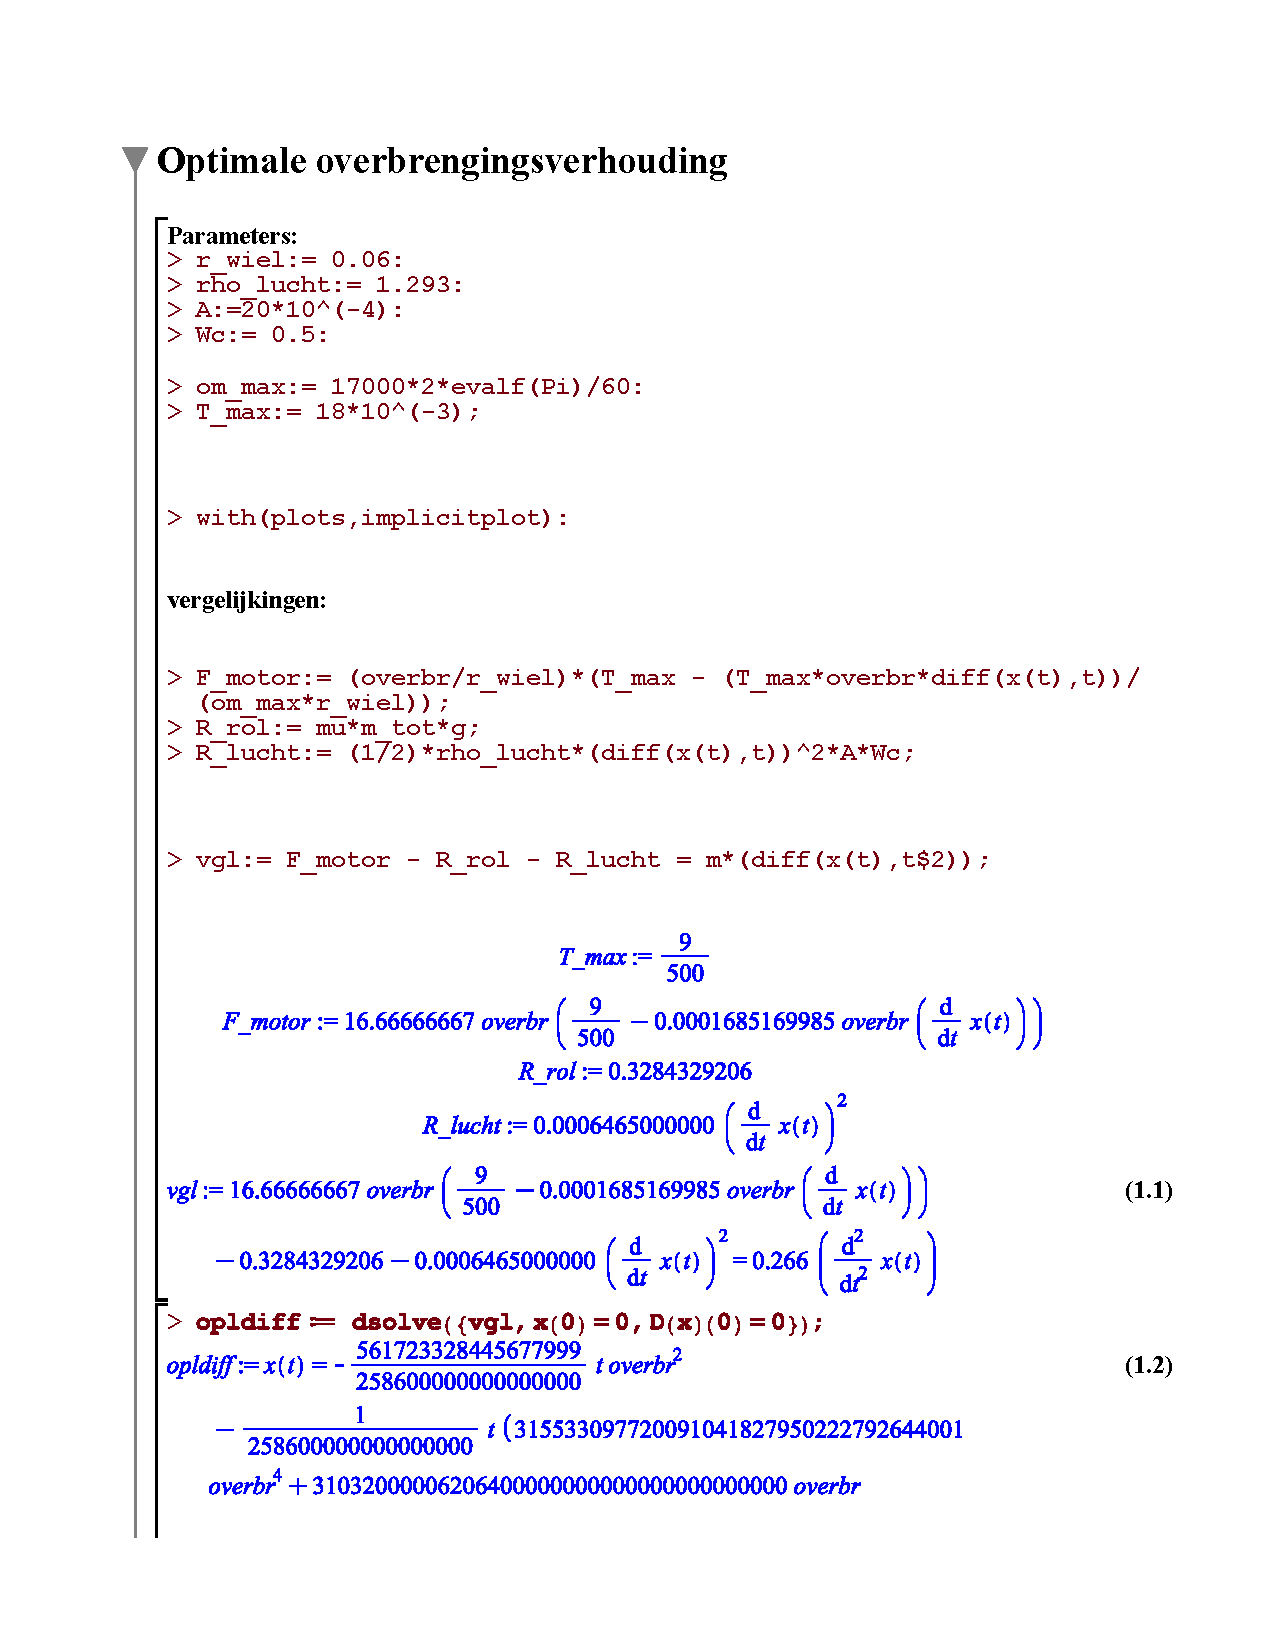
\includepdf[pages={-}]{bijlagen/overbrenging/optimale-overbrenging.pdf}
